\section{Experiments}\label{sec:expe}

Corollary~\ref{thm:finite} makes three concrete predictions. 
First, for a fixed prompt budget $m$, accessibility stays high up to a length threshold $n^\star(m)$, and then the fraction of accessible sequences decays exponentially fast as $n$ increases. 
Second, this threshold grows linearly with the prompt budget, i.e., $n^\star(m)=Cm$ for some $C>0$. 
Third, the corollary provides an explicit upper bound on $C$. 

We first test the first two predictions through the cramming task~\citep{kuratov-etal-2025-cramming} in Section~\ref{sec:cramming}: we measure whether a frozen transformer can generate a target sequence using optimized soft prompts. 
We next refine the theoretical upper bound and compare it to the empirical slope (Section~\ref{sec:support}, ~\ref{sec:cells}).

Finally, we illustrate the saturation regime predicted in Corollary~\ref{thm:wass} using the (easier to compute) copying task.

\begin{figure*}[t]
    \centering
    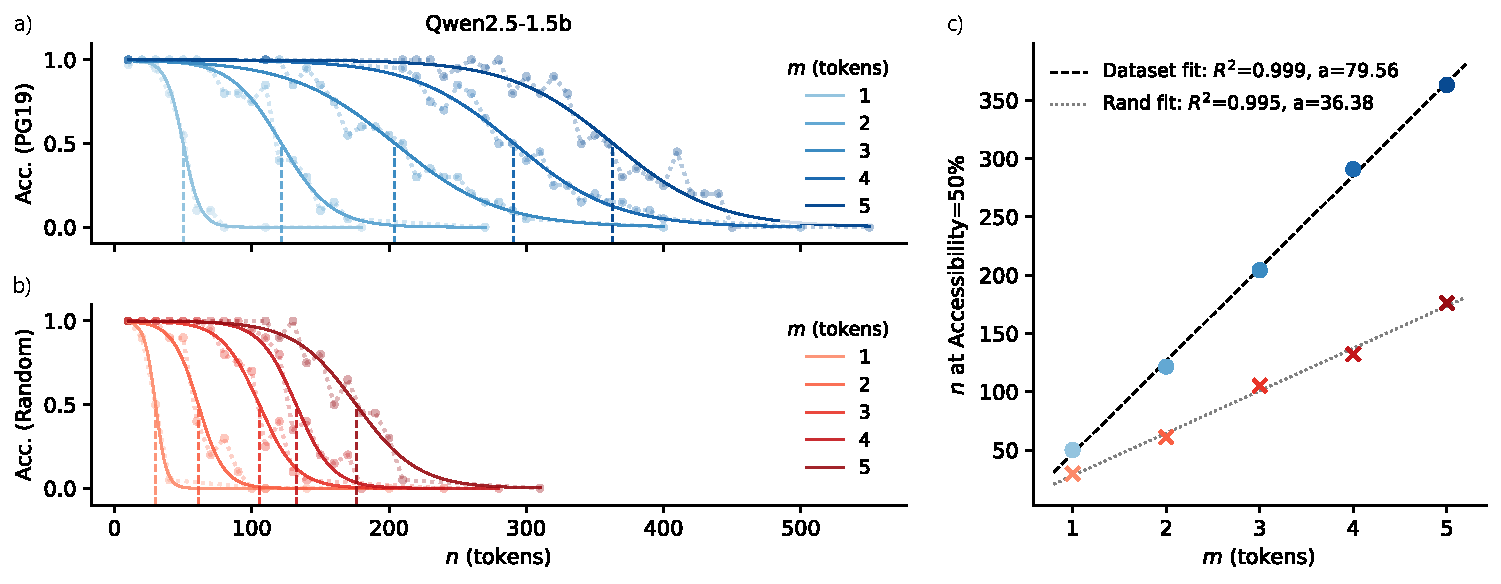
\includegraphics[width=\textwidth]{Images/Qwen_Qwen2.5-1.5B_both.pdf}
    \caption{Mean accessibility for a) PG19 and b) random target sequences of length $n$ as a function of the number of trainable memory vectors $m$. For each $m$, we fit a sigmoid (solid) and mark $n_{50}$ where the fit crosses 0.5 (vertical dashed line). (c) $n_{50}(m)$ for PG19 (blue) and random (red), with linear fits (dashed).}
    \label{fig:exp1}
\end{figure*}

\subsection{The Cramming Task}
\label{sec:cramming}

We want to test whether a target sequence is accessible, i.e., whether there exists some prompt that makes a model generate it. 
Directly searching over discrete prompts is intractable, so we optimize a length-$m$ soft prompt and check for an exact match.
Given a pretrained transformer $\tau$ and a target token sequence $x_{1:n}$, we say the sequence is accessible with prompt length $m$ if there exists a sequence of $m$ soft prompt vectors $Y \in \mathbb{R}^{d \times m}$ such that greedy decoding from $Y$ generates exactly $x_{1:n}$. 
To search for such a prompt, we use the cramming setup of~\citet{kuratov-etal-2025-cramming}: we freeze the model weights and optimize only $Y$ to maximize the likelihood of the target under teacher forcing. Concretely, we minimize the cross-entropy
\begin{equation}
\mathcal{L}(Y; x_{1:n})
= -\sum_{i=1}^{n} \log p_{\tau}\!\left(x_i \mid [Y, x_{1:i-1}]\right),
\label{eq:cramming_loss}
\end{equation}

After optimization, we evaluate accessibility by generating exactly $n$ tokens greedily from the learned prompt $Y$:
\begin{equation}
\hat{x}_i = \arg\max_{t \in \mathcal{V}} p_{\tau}\!\left(t \mid [Y, \hat{x}_{1:i-1}]\right),
\qquad i=1,\dots,n,
\label{eq:greedy_decode}
\end{equation}
and we count a success if $\hat{x}_{1:n}=x_{1:n}$. For each $(n,m)$ we estimate accessibility as the mean success rate over $20$ target strings.
We consider two target sources: i) contiguous token spans of length $n$ sampled from PG19~\citep{rae2019compressive} using each model's tokenizer, and ii) random strings formed by sampling tokens uniformly i.i.d.\ from a subset of the model vocabulary. 

We test whether, for fixed $m$, success stays high up to a length threshold and then drops quickly as $n$ increases; and if this threshold scales roughly linearly with $m$. 
We run the same procedure across several model families and sizes: Pythia (160M, 410M, 1B, 1.4B, 2.8B)~\citep{pmlr-v202-biderman23a}, Qwen-2.5 (0.5B, 1.5B)~\citep{yang2024qwen2}, Llama-3.2 (1B, 3B)~\citep{llama}, and Gemma-3 (270M, 1B)~\citep{gemma}.


\begin{table*}[ht]
\centering
\caption{Ratio between the theoretical upper bound on the slope (using the infinity norm) and the empirical one for natural texts (PG19), across various models. Rows correspond to different enclosure strategies, and columns to the evaluated models. The detailed theoretical analysis is provided in Appendix~\ref{app:shapes}.}
\begin{tabular}{lccccccc}
\toprule
 & \multicolumn{3}{c}{Pythia} & \multicolumn{2}{c}{Qwen-2.5} & Llama-3.2 & Gemma-3 \\[-0.5ex]
\cmidrule(r{2pt}l{2pt}){2-4}\cmidrule(r{2pt}l{2pt}){5-6}\cmidrule(r{2pt}l{2pt}){7-7}\cmidrule(r{2pt}l{2pt}){8-8}
 & 160M & 410M & 1B & 0.5B & 1.5B & 1B & 270M \\[-0.5ex]
\midrule
% Ball & 5.44	& 5.71	& 4.58	& 9.00	& 12.63	& 8.20	& 5.93	 \\
% Cone & 5.29 & 5.52 & 4.51 & 8.88 & 12.49 & 7.85 & 5.66\\
% Ellipsoid &  4.12 & 4.07 & 2.94 & 5.83 & 7.47 & 5.75 & 5.54	\\
% Ellipsoid + Non-uniform Cells &  3.46 & 2.99 & 2.19 & 4.21 & 5.29 & 5.19 & 4.38 \\
Ball & 9.24 & 9.79 & 7.77 & 14.1 & 20.4 & 14.3 & 11.52 \\
Cone & 9.10&  9.60&  7.70&  14.01& 20.34& 13.98& 11.24 \\ 
Ellipsoid & 7.92&  8.15&  6.12&  10.96& 15.30& 11.86& 11.12 \\
Ellipsoid + Non-uniform Cells & \textbf{6.66} & \textbf{5.99} & \textbf{4.56} & \textbf{7.92} & \textbf{10.82} & \textbf{10.71} & \textbf{8.79} \\ 
Ellipsoid + variable $\varepsilon$& 8.65 & 9.83 & 7.71 & 12.32 & 18.81 & 14.63 & 13.42 \\ 


\bottomrule
\end{tabular}
\label{tbl:slope}
\end{table*}

% Our analysis identifies a fundamental limitation in transformer expressivity.
% For every transformer, there exists a critical sequence length beyond which most sequences cannot be generated, no matter the prompt~(Theorems~\ref{thm:wass}~and~\ref{thm:eo}).
% Once this critical length is exceeded, the set of sequences that remain accessible shrinks exponentially with sequence size~(Corollary~\ref{thm:wass}).
% In other words, as inputs grow, transformers lose expressive coverage at an exponential rate, even under ideal training conditions. Remarkably, this theoretical phenomenon is clearly mirrored in empirical behavior.

% In our setting, a sequence is accessible to a transformer if and only if there exists some prompt that makes the model generate that exact sequence as output. 
% The “cramming’’ procedure of~\citet{kuratov-etal-2025-cramming} formalizes this notion: for any target sequence $[\mathbf x_1,\ldots,\mathbf x_n]$, they learn a set of trainable memory vectors $[\mathbf{mem}]=[\mathbf y_1,\ldots,\mathbf y_m]$ which, when used as input to the model, cause it to generate $[\mathbf x_1,\ldots,\mathbf x_n]$. 
% This approach effectively searches over all possible prompts---including highly unnatural ones---to determine whether such a sequence is accessible. 
% Hence, cramming provides an exact operational criterion for accessibility: a sequence is accessible precisely when a corresponding encoding $[\mathbf{mem}]$ exists.

% Following \citet{kuratov-etal-2025-cramming}, we test whether a sequence of $n$ tokens can be encoded into a $[\mathbf{mem}]$ embedding of lengtht $m$ using Pythia-160M~\citep{pmlr-v202-biderman23a}. For each $(n,m)$, we randomly draw 20  target strings of length $n$ from PG19 datatset~\citep{rae2019compressive}, instantiate $m$ trainable embeddings, and optimize them with cross-entropy to maximize the likelihood of the $n$-token target.
% For a target string $x_{1:n}$, we define a success indicator $1\{\hat{x}_{1:n}=x_{1:n}\}$ where $\hat{x}_{1:n}$ is the model’s \emph{greedy} next-token continuation when conditioned only on the learned $m$ tokens. We estimate average accessibility at $(n,m)$ with the mean success rate over 20 strings (1 if exact match, 0 otherwise).

We report Qwen-2.5 (1.5B) results in Figure~\ref{fig:exp1}, results on different model sizes of the same architecture in Appendix~\ref{fig:cram_pythia_suite} and results on different architectures in Appendix~\ref{fig:cram_architectures}.

Figure~\ref{fig:exp1}a reports mean accessibility for natural-language targets (PG19 spans) of length $n$, using memory lengths $m\in\{1,\ldots,5\}$. 
For each fixed $m$, accessibility stays high up to a critical length and then drops sharply. We summarize each curve by fitting a sigmoid; the fits are consistently good (minimum $R^2=0.88$).

Figure~\ref{fig:exp1}b shows the same experiment for random token sequences. Despite being out of distribution, we observe the same pattern: beyond a critical length, accessibility falls rapidly with $n$, consistent with the exponential decay predicted by Corollary~\ref{thm:finite} for fixed $m$.

Figure~\ref{fig:exp1}c plots the length $n$ at which accessibility crosses $0.5$. The scaling is close to linear in both domains ($R^2_{\text{PG19}}=0.999$, $R^2_{\text{rand.}}=0.995$), matching the linearity prediction of Corollary~\ref{thm:finite}. The slope differs between domains: PG19 targets remain accessible for longer than random strings at the same $m$. A likely reason is that natural text has structure the model can exploit, so the effective amount of information to store is smaller; a similar gap was reported by~\citet{kuratov-etal-2025-cramming}.

In addition, the theoretical slope from Corollary~\ref{thm:finite} is a close upper bound on the slopes estimated from Figure~\ref{fig:exp1}c (first row of Table~\ref{tbl:slope}), as the factor is between $5$ and $10$. 
The small gap is expected: Corollary~\ref{thm:finite} is an upper bound and relies on simplifying geometric assumptions. 
In particular, it assumes that 
i) the embedding support is a fully used ball of radius $r$, and 
ii) each token sequence $\mathbf t$ corresponds to a region $\mathcal{E}_{\mathbf t}$ of equal volume in the embedding space. 

In the following, we relax these worst-case assumptions by better approximating the embedding support $\mathcal{E}$ (Section~\ref{sec:support}) and by empirically estimating the distribution of cell volumes $|\mathcal{E}_{\mathbf t}|$ (Section~\ref{sec:cells}).

\subsection{Support Refinement}
\label{sec:support}

Prior work shows that transformer embeddings occupy a small and anisotropic subset of the $d$-dimensional ball of radius $r$, rather than filling it uniformly~\citep{rudman-etal-2022-isoscore}. 
This matters for our bound: if the effective support is smaller than the full ball volume, the accessibility threshold $n^\star(m)$ should be reached at smaller $n$, which lowers the predicted slope.

We upper bound the support by enclosing it within two simple shapes that capture anisotropy: an axis-aligned ellipsoid and a cone. We compute the corresponding packing numbers for each shape and plug them into the slope bound; derivations are deferred to Appendix~\ref{app:shapes}. 
Computing packing numbers requires the radius $r$ for the ball, per-dimension radius $r_i$ for the ellipsoid, and the smallest opening angle that contains all sampled embeddings for the cone. We estimate these support-dependent parameters by Monte Carlo using 10K prompts of length at most $\ell$, generated by sampling tokens i.i.d.\ from the model vocabulary and concatenating them, and mapping each prompt to an embedding using the same extraction procedure as in the main cramming setup. Experimental details are in Appendix~\ref{app:support}, and the effect of $\ell$ on the resulting upper bounds is shown in Figure~\ref{fig:support}. In practice, $\ell \approx 1000$ tokens is sufficient to obtain a stable upper-bound estimate.

Using cone or ellipsoid supports, we recompute the theoretical slope and compare it to the empirical slope from Figure~\ref{fig:exp1}c. The updated ratios are reported in Table~\ref{tbl:slope} (rows 2 and 3). The gap shrinks for all models, while remaining slightly larger for Qwen-2.5-1.5B.

\subsection{Cell Volume Distribution}
\label{sec:cells}

\begin{figure}[t]
    \centering
    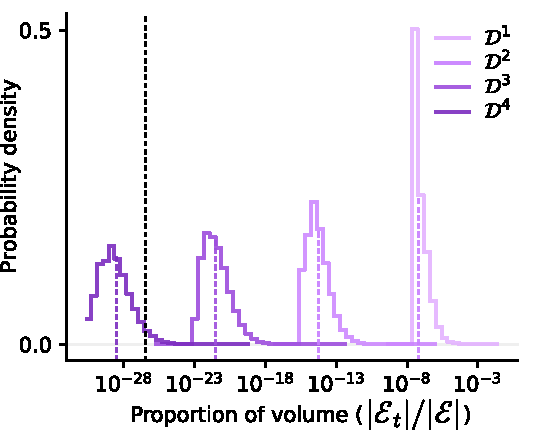
\includegraphics[width=0.40\textwidth]{Images/concept_convolution.pdf}
    \caption{Conceptual example of using the cell-volume distribution to tighten the upper bound. Rather than assuming equal-volume cells (Dirac mass), we take the $n$-fold convolution of the empirical one-step volume distribution $\mathcal{D}^1$ (light violet) and track when the median of $\mathcal{D}^n$ (violet dashed) drops below the threshold (black dashed).}
    \label{fig:convolution}
\vspace{-1.5em}
\end{figure}


Corollary~\ref{thm:finite} makes an equal-volume approximation: each token (or sequence) corresponds to a region of the embedding space $\mathcal{E}_{\mathbf t}$ of equal size. In practice this is unlikely. Common tokens should occupy larger regions under the model's decoder, while rare or specialized tokens may correspond to much smaller regions. 
Here we measure how uneven these decoder cell volumes are by considering the empirical distribution $\mathcal D$ of the cell volumes of every token $t$ in terms of proportion $\frac{\lvert \mathcal{E}_t \rvert}{|\mathcal E|}$.

Concretely, we first approximate the distribution $\mathcal D$ corresponding to the next token, then study the $n$-fold multiplicative convolution $\mathcal D^{n}$ to model the distribution of the next $n$ tokens. We compute the smallest $n$ such that the median of $\mathcal D^{n}$ falls below $\frac1{\mathcal{P}(\mathcal E,\|\cdot\|,\varepsilon)}$, that is when at least half of the sequences become inaccessible (see Figure~\ref{fig:convolution} for a conceptual example). We describe how we obtain the volumes $\lvert \mathcal{E}_{\mathbf t} \rvert$ in Appendix~\ref{app:cell_vol}.

\begin{remark}
    In the uniform setting underlying Corollary~\ref{thm:finite}, the distribution $\mathcal D$ collapses to a Dirac mass at $\frac{1}{ \lvert \mathcal V \rvert}$, reflecting equal-volume cells for all tokens.
    Note that the procedure described above exactly recovers the bound of Corollary~\ref{thm:finite}, while nontrivial dispersion in $\mathcal D$ yields strictly sharper, data-dependent limits.
\end{remark}

Combining this with the ellipsoid support, we recompute the theoretical slope and compare it to the empirical slope from Figure~\ref{fig:exp1}c. The updated ratios are reported in Table~\ref{tbl:slope} (row 4). The gap shrinks for all models.

\begin{remark}
    The assumption of uniform precision $\varepsilon$ may be too restrictive. We therefore provide a more refined analysis, whose results are reported in the last row of Table~\ref{tbl:slope}. Details are given in Appendix~\ref{app:epsilon}. Although the resulting upper bounds remain valid, they do not account for the fact that most internal representations lie far from $0$, which leads to looser bounds in practice.
\end{remark}

\subsection{Copying-Length Generalization.}

% \begin{table*}[ht]
% \centering
% \caption{Copying task performance (mean with standard deviation in parentheses) across evaluation lengths.}
% \begin{tabular}{lrrrrr}
% \toprule
%  & \multicolumn{5}{c}{Eval length} \\[-0.5ex]
% \cmidrule(lr){2-6}
% Model & 50 & 100 & 200 & 300 & 400 \\[-0.5ex]
% \midrule
% Pythia-1.4B & 1.00 (0.00) & 0.92 (0.06) & 0.04 (0.06) & 0.00 (0.00) & 0.00 (0.00) \\
% Pythia-1B   & 1.00 (0.00) & 1.00 (0.00) & 0.42 (0.06) & 0.08 (0.06) & 0.00 (0.00) \\


% \bottomrule
% \end{tabular}
% \label{tbl:copying_lengths}
% \end{table*}


\begin{figure}[t]
    \centering
    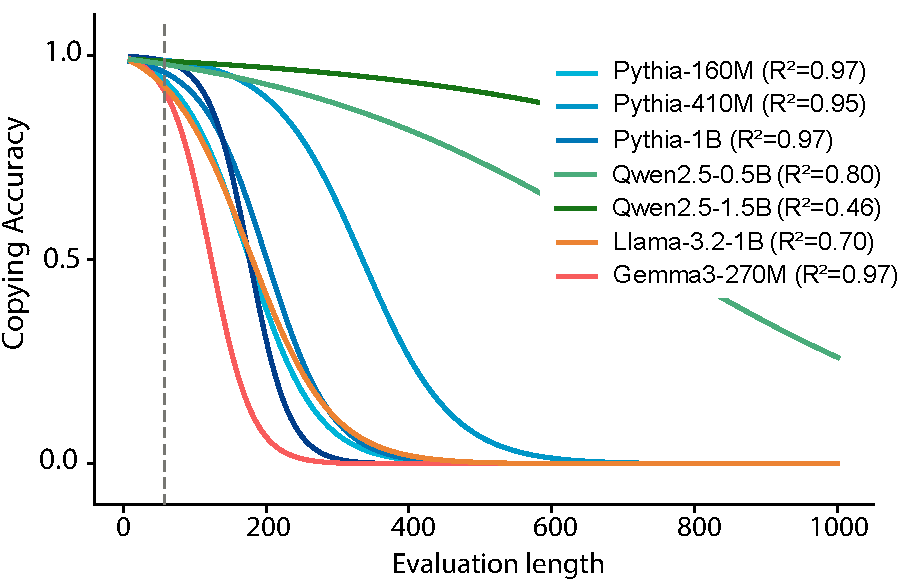
\includegraphics[width=0.45\textwidth]{Images/copying_synthetic_parent_results_fit_only.pdf}
    \caption{Models are trained to copy strings up to a maximum length (grey dashed) and evaluated on generating the exact copy of longer strings. We report exact-match copying accuracy versus string length. For each model, we fit a sigmoid to the accuracy curve (continuous lines) and report the corresponding $R^2$.}
\vspace{-2.5em}
    \label{fig:copying}
\end{figure}


% In the first part of this section, we concentrated on the theoretical predictions of Corollary~\ref{thm:finite}, which can be directly confronted with empirical behavior via the cramming task. However, cramming becomes prohibitively expensive as the prompt length $m$ grows, making empirical evaluation of Theorem~\ref{lem:wass} impractical. 
% We therefore turn to the copying task: since Corollary~\ref{thm:wass} predicts that, beyond a certain length threshold, most sequences are inaccessible to a fixed transformer $\tau$, it should in particular be impossible for $\tau$ to copy such sequences.
The first part of this section tested the predictions of Corollary~\ref{thm:finite} using the cramming task. As prompt length $m$ grows, cramming becomes prohibitively expensive, so we evaluate Corollary~\ref{thm:wass} through the copying task instead. Corollary~\ref{thm:wass} predicts a length threshold beyond which most sequences are inaccessible to a fixed transformer $\tau$; it should in particular be impossible for $\tau$ to copy such sequences. Moreover, as for Corollary~\ref{thm:finite}, a sharp decline in proportion of accessible sequences is predicted past this threshold.

We test this directly by adding a copying-length generalization experiment following~\citet{meyer2025memorylimitationsprompttuning}, avoiding expensive cramming experiments. We fine-tune pretrained 
% Pythia-1B and Pythia-1.4B
models on a synthetic exact string-copying task using next-token cross-entropy loss. 
Training examples are random strings $x_{1:n}$ of length at most $50$, formatted as $x_{1:n}\mid x_{1:n}$, where the model is conditioned on the prefix $x_{1:n}\mid$ and trained to generate the target copy $x_{1:n}$. 
Training stops at $100\%$ exact-match accuracy on length $50$ or after $10$K optimization steps 
We then evaluate exact-match copying accuracy on longer unseen strings within the model context window.

Figure~\ref{fig:copying} shows a sharp length-dependent transition. Accuracy stays near 100\% on short strings, then falls abruptly once string length exceeds a model-specific threshold. Sigmoid fits capture this transition well, with median $R^2 = 0.95$ across models.

These results suggest that the linear regime observed in Figure~\ref{fig:exp1}b does not continue indefinitely; every transformer admits an accessibility limitation, independent of the prompt length $m$.